%!TEX root = ../report.tex
\chapter{Improving Automated Build}
For this sprint we have chosen to work on four user stories that should improve automated building.

\begin{chapterorganization}
  \item in \sectionref{sec:jenkins_restruct} we explain how we restructure jobs in Jenkins to ease further configuration needs;
  \item in \sectionref{sec:monkey_testing_s2} we describe our work towards making monkey testing work;
  \item in \sectionref{sec:s3_appinstallationtest} we set up a test case that installs all apps on the same device to check if apps are compatible, since this has been an issue;
  \item in \sectionref{sec:s3_linecoverage} we enable generation of a code coverage report and set up showing lines of code covered in Jenkins;
  \item in \sectionref{sec:upload_google_play} we automatically upload successful builds to the Google Play alpha channel.
\end{chapterorganization}

\section{Restructuring Jenkins}\label{sec:jenkins_restruct}
The setup of Jenkins used in sprint 1 was tedious to work with since all jobs were configured independently. If a change had to be made to several jobs, we would have to manually configure the change in each job. Not only did this take a considerable amount of time, but it was also prone to human errors during the process. In this sprint, we have to make small modifications to all jobs several times. This would be very tedious, so we have decided make job configurations easier to manage, even though it is not connected directly to a story. We consider it refactoring.

The jobs on Jenkins are generally very similar in their configuration. We can benefit from having a base configuration, which the jobs only modify. There exists a Jenkins plug-in for this, called inheritance-plugin \parencite{jenkins-inheritance}. With this plug-in installed, whenever we decide to make a change to e.g.\ the build system, it will not be necessary to change this in each job. Instead, the change can be made on the base job, and all relevant jobs will inherit this change. This also ensures that jobs follow a consistent pipeline and thus do not differ in from job to job.

The plug-in requires the jobs to be of a special \emph{inheritable} type. We therefore have to covert the existing jobs to inheritable jobs to take advantage of this. As it is impossible to convert a existing job to the inheritable type, we have to re-create all the jobs again. This is not that big of a deal, as the time to setup will be considerably shorter when taking advantage of the inheritable job type. When the old jobs are removed the build history will be lost. This is a minor nuisance but we consider it a small price to pay, compared to the advantages. When deciding how to structure the build, we see two general categories that are sufficiently distinct: Android apps and Android libraries. We create an abstract job for each of these. They do overlap somewhat in functionality, which means we have to create an abstract job for each job task. As such we create abstract jobs for e.g.\ \emph{run Gradle}, \emph{run unit tests}, \emph{find and move APKs}, and \emph{publish lint report} \kimnote{Disse navne skulle fremgå af figuren}. The abstract jobs \emph{Android app} and \emph{Android library} inherit from the small abstract tasks that are relevant.

We have modeled this as a diagram in \figureref{fig:jenkins_inherit}.

\begin{figure}%
\centering
\tikzsetnextfilename{jenkins_inherit}
\begin{tikzpicture}[
  simple/.style={draw, rounded corners, minimum height=1.8em},
  simplefixed/.style={draw, rounded corners, minimum height=1.8em, minimum width=10em},
  square/.style={draw, rounded corners, minimum height=1.4em, minimum width=1.4em}]
  
  \begin{scope}[]
    \matrix[column sep=.5cm]{
      \node[simple] (pubAPK) {Publish APK}; &
      \node[simple] (email) {Email}; &
      \node[simple] (coco) {CoCo}; &
      \node[] (dots) {\dots};  &
      \node[simple] (emu) {Emulator}; &
      \node[simple] (pubLib) {Publish lib}; \\
    };
  \end{scope}
  
  \begin{scope}[yshift=-2cm]
    \matrix[column sep=1.5cm]{
      \node[simplefixed] (appInh) {App Inheritable}; &
      \node[simplefixed] (libInh) {Lib Inheritable}; \\
    };
  \end{scope}
  
  \begin{scope}[yshift=-3.5cm]
    \matrix[column sep=.3cm]{
      \node[simple] (app1) {App 1}; &
      \node[simple, right=of app1] (app2) {App 2}; &
      \node[right=of app2] (dots) {\dots}; &
      \node[simple, right=of dots] (appn) {App $n$}; &
      \node[] (dummy) {}; &
      \node[] (dummy2) {}; &
      \node[simple] (lib1) {Lib 1}; &
      \node[simple, right=of lib1] (lib2) {Lib 2}; &
      \node[right=of lib2] (dots) {\dots}; &
      \node[simple, right=of dots] (libn) {Lib $n$}; \\
    };
  \end{scope}

  \draw[<-] (appInh) to (app1);
  \draw[<-] (appInh) to (app2);
  \draw[<-] (appInh) to (appn);
  \draw[<-] (libInh) to (lib1);
  \draw[<-] (libInh) to (lib2);
  \draw[<-] (libInh) to (libn);
  
  \draw[<-] (pubAPK) to (appInh);
  \draw[<-] (email) to (appInh);
  \draw[<-] (coco) to (appInh);
  \draw[<-] (emu) to (appInh);
  
  \draw[<-] (pubLib) to (libInh);
  \draw[<-] (email) to (libInh);
  \draw[<-] (coco) to (libInh);
  \draw[<-] (emu) to (libInh);
        
  \draw[decorate, line width=1pt, decoration={brace, mirror}] ([xshift=1.5em]pubLib.south east) -- ([xshift=1.5em]pubLib.north east) node [midway, yshift=0em, xshift=2.7em] {Sub-tasks};
  
  %\draw[decorate, line width=1pt, decoration={brace, mirror}] ([xshift=1.5em]bd.south east) -- ([xshift=1.5em]bd.north east) node [midway, yshift=-0.1em, xshift=3.2em] {Subprojects};
  
\end{tikzpicture}
\caption{Jenkins inheritable jobs}%
\label{fig:jenkins_inherit}%
\end{figure}

\section{Monkey Testing}\label{sec:monkey_testing_s2}
During sprint 1 we encountered some difficulties related to monkey testing. In order to monkey test we need to install the apps on an Android device, but we did not have these easily available\kimnote{rephrase, make it clear that you talk about the apps that need to be monkey tested.}. As described in \chapterref{sec:upload_google_play} the signed APKs for each app is now stored on the ftp sever. As the ftp server is hosted on the same machine as Jenkins, we can directly access the APKs from the directory. To install we simply need to identify the newest build of each app, as, for now, the old builds are kept as well.  

To install a specific app to an Android device, we use the script seen in \listingref{lst:find_newest_apk}, parsing to it the application id of the app. All APKs containing the given application id is then found. This result is piped to \code{sed 's|.*b||' |'s|\_release\_aligned.apk||' }\kimnote{consider changing the separation symbol in sed such that it is not the same as pipe.} that removes everything but the build number of the files. \code{awk '\$0>x\{x=\$0\};END\{print x\}'} then finds the maximum build number. Finally the newest APK for the given application id is found.

\begin{lstlisting}[language=bash,showstringspaces=false,caption=Script that finds the newest build number for a particular application id,label=lst:find_newest_apk]
NEWEST_BUILD="$(find /srv/ftp/newest_apks/ -name "$1*release_aligned.apk" | sed 's|.*b||' | sed 's|_release_aligned.apk||' | awk '$0>x{x=$0};END{print x}')"
find /srv/ftp/newest_apks/ -name "$1*b${NEWEST_BUILD}_release_aligned.apk"
\end{lstlisting}

When the app has been installed on the device, we run a monkey test on it using the Jenkins plugin. Starting a monkey test will launch the app. This poses problems for the majority of the Giraf apps, as they require extra information when starting, such as user information. If the apps are not given this information at launch they will crash. This means that all monkey tests report failure. The only app that require no extra information is the launcher. However, as the launcher uses the first 5--10 minutes downloading pictograms, the monkey test only presses on a loading screen.

The \mono{monkey} command does not support sending extra information when starting apps. We did not anticipate this obstacle and did therefore not manage to implement monkey testing for apps fully.

\section{App Installation Test Case}\label{sec:s3_appinstallationtest}
To ensure that all apps of the multi-project are compatible a test on Jenkins is run nightly that installs all apps on a single device. At the end of sprint 1 the GUI groups had issues installing a combination of apps on a single device --- this test case should avoid such an issue in the future.

To do this we find the newest version of all available APKs on the server. These APKs are the same that are uploaded to Google Play. The script seen in \listingref{lst:find_all_newest_apks} finds the application id for each available app by finding all files in the directory containing APKs. It then pipes these files to \code{sed 's|.*/||'} which removes the path of the file. This is then piped to \code{sed 's|\_v.*||'} that removes everything following the package id. The output of that is then sorted and all duplicates are removed using \code{sort | uniq}. The sort is necessary as \mono{uniq} only removes duplicate lines that are adjacent. 

The application names are then send to \mono{find\_newest\_apk.sh}, as seen previously in \listingref{lst:find_newest_apk}.

\begin{lstlisting}[language=bash,showstringspaces=false,caption=Script that finds the newest available APK for all apps,label=lst:find_all_newest_apks]
PACKAGE_NAMES="$(find /srv/ftp/newest_apks/ -name "*release_aligned.apk" | sed 's|.*/||' | sed 's|_v.*||' | sort | uniq)"


for p in $PACKAGE_NAMES
do
    /srv/scripts/find_newest_apk.sh $p
done
\end{lstlisting}

When the newest available APK for each app has been found, they are installed on an Android device. Line 3 tries to install an APK and stores the output in \mono{INSTALL\_OUTPUT}\kimnote{remember to reference install\_apks\_on\_android\_device}. The output is stored, as \mono{adb install} gives an error code of 0, even if it fails. We therefore have to read the output to check if an error occurred so that Jenkins will report the job as a failure. This is done at line 6 where we check that the output contains the string \mono{success}. The \mono{-i} option makes \mono{grep} case insensitive. At line 9--10 we exit with 1 if the output does not contain \mono{success}.

\begin{lstlisting}[language=bash,showstringspaces=false,caption=Script that installs the given APKs to an Android device,label=lst:install_apks_on_android_device]
for a in $@
do
    INSTALL_OUTPUT="$(/srv/android-sdk-linux//platform-tools/adb install $a)"
    echo $INSTALL_OUTPUT

    IS_SUCCESS="$(echo "$INSTALL_OUTPUT" | grep -i success)"

    # Check if output message does not contain success, since adb install does not provide exit code != 0 at failure
    if ! [ "$IS_SUCCESS" ]; then
        echo "Error installing $a"
        exit 1
    fi
done
\end{lstlisting}

If the installation of any app fails on the device, the Jenkins job will fail.

\section{Code Coverage Reports}\label{sec:s3_linecoverage}
We have a user story which states that Jenkins should provide code coverage metrics for every project. This user story was generated by a group which was writing test of a database project and wanted a measure of their progress. Their main request is for a percentage of lines of code covered. A tool for code coverage report must at least provide this metric, but other more detailed metrics will also be nice to have. In version 0.10 of the \emph{New Android SDK Build System} \parencite{new-build-android}, support for the JaCoCo \parencite{jacoco-home} Java Code Coverage Library was included. It meets all of our demands for metrics and is nicely integrated into the Android and Gradle build system. To make JaCoCo generate a report all one needs to do is to add the code shown in \listingref{lst:Jacoco} to the \mono{build.gradle} file of the project.

\begin{gradlecode}[caption=Gradle script for enabling JaCoCo,label=lst:Jacoco]
dependencies {
    mavenCentral()
}
android {
    buildTypes {
        debug {
            testCoverageEnabled true
        }
    }
}
\end{gradlecode}{}
\kimnote{Config files are not very interesting, this also applies to maven configs. Only add them if you did something smart or complex. I suggest that you remove them from your report.}

Now we generate code coverage reports for debug builds locally and in Jenkins. We would like to also publish the code coverage results in Jenkins. There exists a Jenkins plugin \parencite{jacoco-jenkins-plugin} for this purpose. This plugin is easy to setup, provides detailed coverage statistics, and an overview with the percentage of lines of code covered. We use this plugin for publishing the code coverage metrics in Jenkins. An example of this can be seen in \figureref{fig:jenkins-overview-coco}

\begin{figure}[htbp]
    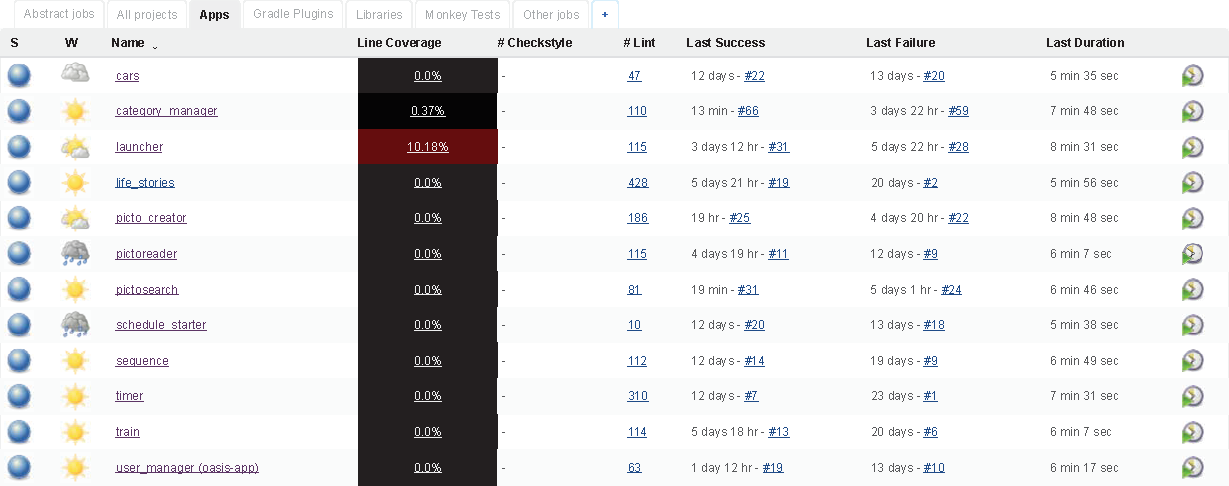
\includegraphics[width=\textwidth]{graphics/jenkins-overview-coco.pdf}
    \caption{Screenshot of a section of the build overview screen which shows the code coverage column}
    \label{fig:jenkins-overview-coco}
\end{figure}